\section{Estudio de las especificaciones}
    \subsection{Dominio del problema}

    El dominio de este problema engloba a todas las personas con discapacidad auditiva que puedan requerir el uso del sistema a implementar. Para tratar el problema en cuestión, se realiza una entrevista con un grupo de personas con esta discapacidad.

    \subsection{Selección de personas a entrevistar}

    Para la obtención de unos datos ajustados a la realidad, se entrevista a personas con discapacidad auditiva pertenecientes a la asociación ``Albor Cádiz'', de la que hay disponible más información en su página de Facebook: \url{https://www.facebook.com/alborcadiz}.

    \subsection{Objetivo y contenido de la entrevista}

    El objetivo de esta entrevista es el de obtener los requisitos del sistema, de la manera más real posible. El contenido de la entrevista se puede encontrar en el apartado~\ref{sec:cuestionario} del Anexo.

    \subsection{Planificación de la entrevista}

    La entrevista se realiza el día 29 de Abril de 2015, a las 18:30 horas, en la sede de la asociación ``Albor Cádiz''.

    \subsection{Análisis de los resultados obtenidos en la entrevista}

    \begin{itemize}
        \item[\textbf{1}] \textbf{¿Qué avisos son importantes para ti en tu hogar?}\\
            En la figura~\ref{fig:resultados1} se puede observar como las alertas de mayor interés son las llamadas a la puerta (timbre) o al telefonillo, además de varias sugerencias para otros avisos. Queda así descartado el control de alertas para llamadas de teléfono, pues no supone gran interés.
            \begin{figure}[!ht]
            \centering
                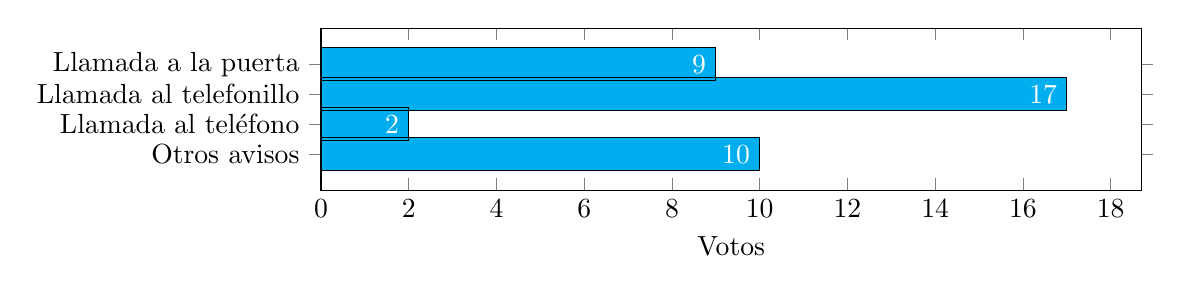
\begin{tikzpicture}
                    \begin{axis}[
                        xbar,
                        bar width=\baselineskip,
                        xmin=0.0,
                        width=12cm,
                        height={.3\textwidth},
                        ytick={1,2,3,4},
                    	yticklabels={{Otros avisos},{Llamada al teléfono},{Llamada al telefonillo},{Llamada a la puerta}},
                    	enlarge y limits=0.4,
                    	xlabel={Votos},
                    	ytick=data,
                    	nodes near coords,
                        nodes near coords align=left,
                        every node near coord/.style={color=white}
                    ]
                    \addplot [draw=black, fill=cyan] coordinates {
                        (10, 1)
                        (2, 2)
                        (17, 3)
                        (9, 4)
                    };
                    \end{axis}
                \end{tikzpicture}
                \caption{Resultados para ``¿Qué avisos son importantes para ti en tu hogar?''}
                \label{fig:resultados1}
            \end{figure}
        \item[\textbf{2}] \textbf{En la actualidad, ¿cómo te percatas de estos avisos?}\\
            Se observa en la figura~\ref{fig:resultados2} los resultados para esta pregunta. La mayoría de los encuestados utilizan actualmente sistemas de alertas mediante luces.
            \begin{figure}[!ht]
            \centering
                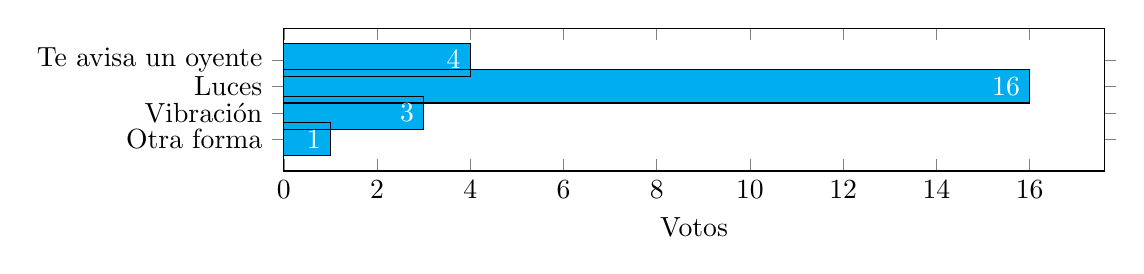
\begin{tikzpicture}
                    \begin{axis}[
                        xbar,
                        bar width=\baselineskip,
                        xmin=0.0,
                        width=12cm,
                        height={.28\textwidth},
                        ytick={1,2,3,4},
                    	yticklabels={{Otra forma},{Vibración},{Luces},{Te avisa un oyente}},
                    	enlarge y limits=0.4,
                    	xlabel={Votos},
                    	ytick=data,
                    	nodes near coords,
                        nodes near coords align=left,
                        every node near coord/.style={color=white}
                    ]
                    \addplot [draw=black, fill=cyan] coordinates {
                        (1, 1)
                        (3, 2)
                        (16, 3)
                        (4, 4)
                    };
                    \end{axis}
                \end{tikzpicture}
                \caption{Resultados para ``En la actualidad, ¿cómo te percatas de estos avisos?''}
                \label{fig:resultados2}
            \end{figure}
        \item[\textbf{3}] \textbf{Haciendo uso de las nuevas tecnologías, ¿crees que puede mejorarse?, ¿cómo te gustaría percatarte de los avisos?}\\
            Los resultados para esta pregunta se exponen en la figura~\ref{fig:resultados3}. La mayoría de los encuestados prefieren alertas con luces, en concreto, de colores y parpadeantes, según comentan; además de vibraciones, esta última forma genera cierto rechazo ya que puede sobresaltar al usuario.
            \begin{figure}[!ht]
            \centering
                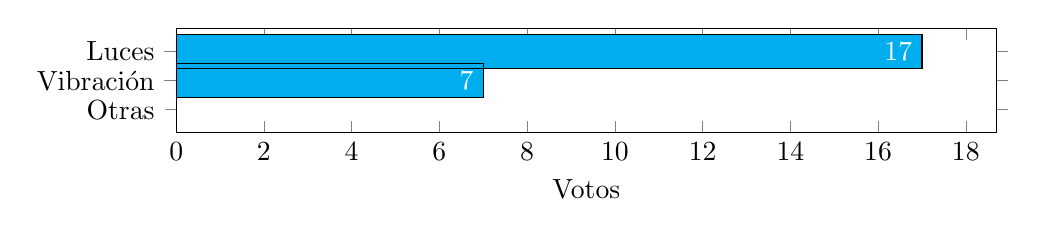
\begin{tikzpicture}
                    \begin{axis}[
                        xbar,
                        bar width=\baselineskip,
                        xmin=0.0,
                        width=12cm,
                        height={.24\textwidth},
                        ytick={1,2,3},
                    	yticklabels={{Otras},{Vibración},{Luces}},
                    	enlarge y limits=0.4,
                    	xlabel={Votos},
                    	ytick=data,
                    	nodes near coords,
                        nodes near coords align=left,
                        every node near coord/.style={color=white}
                    ]
                    \addplot [draw=black, fill=cyan] coordinates {
                        (0, 1)
                        (7, 2)
                        (17, 3)
                    };
                    \end{axis}
                \end{tikzpicture}
                \caption{Resultados para ``Haciendo uso de las nuevas tecnologías, ¿crees que puede mejorarse?,¿cómo te gustaría percatarte de los avisos?''}
                \label{fig:resultados3}
            \end{figure}
        \item[\textbf{4}] \textbf{Continuando con las nuevas tecnologías, ¿crees que sería útil recibir las mismas alertas en smartphones Android?}\\
            Para esta última pregunta, en la figura~\ref{fig:resultados4} se observan los resultados obtenidos. Casi todos los discapacitados encuestados prefieren recibir las mismas alertas en sus smartphones Android, apostando por el uso de aplicaciones para estas alertas.
            \begin{figure}[!ht]
            \centering
                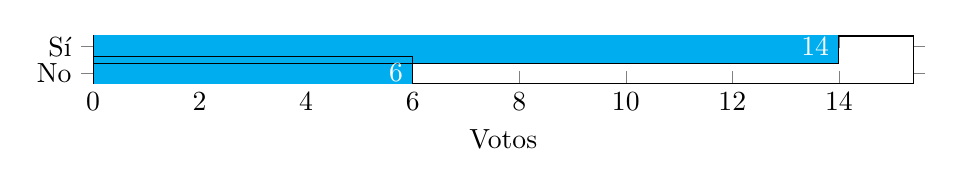
\begin{tikzpicture}
                    \begin{axis}[
                        xbar,
                        bar width=\baselineskip,
                        xmin=0.0,
                        width=12cm,
                        height={.18\textwidth},
                        ytick={1,2},
                    	yticklabels={{No},{Sí}},
                    	enlarge y limits=0.4,
                    	xlabel={Votos},
                    	ytick=data,
                    	nodes near coords,
                        nodes near coords align=left,
                        every node near coord/.style={color=white}
                    ]
                    \addplot [draw=black, fill=cyan] coordinates {
                        (6, 1)
                        (14, 2)
                    };
                    \end{axis}
                \end{tikzpicture}
                \caption{Resultados para ``Continuando con las nuevas tecnologías, ¿crees que sería útil recibir las mismas alertas en smartphones Android?''}
                \label{fig:resultados4}
            \end{figure}
    \end{itemize}

    En cualquier caso, los resultados no están lejos de los esperados, llegando así en resumen a las siguientes conclusiones:
    \begin{itemize}
        \item Los avisos tratados serán las llamadas a la puerta de la vivienda (timbre) y las llamadas al telefonillo o portero automático.
        \item Los avisos se tratarán como alertas visuales mediante luces de colores.
        \item Además de las luces, se desarrollará una aplicación para Android en la que se notifiquen las mismas alertas, ya que es el sistema operativo para smartphone más extendido en el mercado.
    \end{itemize}

\section{Descripción del problema}
    \begin{itemize}
        \item El usuario tiene una discapacidad auditiva.
        \item El usuario necesita percatarse de las alertas sonoras que se dan en el entorno de alguna manera.
        \item Las alertas serán: llamada al telefonillo y llamada al timbre de la puerta de la vivienda.
        \item Las alertas se deben conectar a un sistema.
        \item El sistema alertará visualmente al usuario mediante luces de colores, y mostrando notificaciones en su smartphone.
    \end{itemize}\vspace{-\baselineskip}\mbox{}

\section{Objetivos del sistema}
    \begin{table}[!ht]
        \centering
        \resizebox{\textwidth}{!}{%
       \begin{tabular}{|l|p{11cm}|}
            \hline
            \textbf{OBJ-01} & Alertar a usuario de llamada al timbre. \\ \hline
            \textbf{Descripción} & El sistema deberá alertar visualmente mediante el cambio de color de las luces y mediante notificación vía smartphone de la llamada al timbre al usuario. \\ \hline
            \textbf{Importancia} & Alta. \\ \hline
            \textbf{Estabilidad} & Alta. \\ \hline
            \textbf{Comentarios} & Ninguno. \\ \hline
        \end{tabular}
        }
        \caption{Objetivo 1 del sistema: Alertar a usuario de llamada al timbre.}
        \label{OBJ01}
    \end{table}

    \begin{table}[H]
        \centering
        \resizebox{\textwidth}{!}{%
       \begin{tabular}{|l|p{11cm}|}
            \hline
            \textbf{OBJ-02} & Alertar a usuario de llamada al telefonillo. \\ \hline
            \textbf{Descripción} & El sistema deberá alertar visualmente mediante el cambio de color de las luces y mediante notificación vía smartphone de la llamada al telefonillo al usuario. \\ \hline
            \textbf{Importancia} & Alta. \\ \hline
            \textbf{Estabilidad} & Alta. \\ \hline
            \textbf{Comentarios} & Ninguno. \\ \hline
        \end{tabular}
        }
        \caption{Objetivo 2 del sistema: Alertar a usuario de llamada al telefonillo.}
       \label{OBJ02}
    \end{table}

\section{Requisitos de información}
    \begin{table}[!ht]
        \centering
        \resizebox{\textwidth}{!}{%
       \begin{tabular}{|l|p{11cm}|}
            \hline
            \textbf{CRQ-01} & Relación entre alertas. \\ \hline
            \textbf{Objetivos asociados} & \vspace{-2mm}\begin{itemize}[noitemsep,nosep]
                                                \item OBJ-01 Alertar a usuario de llamada al timbre.
                                                \item OBJ-02 Alertar a usuario de llamada al telefonillo.
                                            \end{itemize}\vspace{-\baselineskip}\mbox{} \\ \hline
            \textbf{Requisitos asociados} & \vspace{-2mm}\begin{itemize}[noitemsep,nosep]
                                                \item IRQ-01 Información de alertas.
                                            \end{itemize}\vspace{-\baselineskip}\mbox{}\vspace{-\baselineskip}\mbox{} \\ \hline
            \textbf{Descripción} & Solo se podrá mostrar una alerta a la vez.  \\ \hline
            \textbf{Importancia} & Alta. \\ \hline
            \textbf{Estabilidad} & Alta. \\ \hline
        \end{tabular}
        }
        \caption{Requisitos de restricciones de información.}
        \label{CRQ01}
    \end{table}

    \begin{table}[!ht]
        \centering
        \resizebox{\textwidth}{!}{%
       \begin{tabular}{|l|p{5cm}|p{5cm}|}
            \hline
            \textbf{IRQ-01} & \multicolumn{2}{|p{10cm}|}{Información de alertas.} \\ \hline
            \textbf{Objetivos asociados} & \multicolumn{2}{|p{10cm}|}{\vspace{-2mm}\begin{itemize}[noitemsep, nosep]
                                                \item OBJ-01 Alertar a usuario de llamada al timbre.
                                                \item OBJ-02 Alertar a usuario de llamada al telefonillo.
                                            \end{itemize}\vspace{-\baselineskip}\mbox{}} \\ \hline
            \textbf{Requisitos asociados} & \multicolumn{2}{|p{10cm}|}{\vspace{-2mm}\begin{itemize}[noitemsep,nosep]
                                                \item UC-01 Alertar timbre.
                                                \item UC-02 Alertar telefonillo.
                                                \item UC-03 Mostrar alerta.
                                            \end{itemize}\vspace{-\baselineskip}\mbox{}} \\ \hline
            \textbf{Descripción} & \multicolumn{2}{|p{10cm}|}{El sistema deberá alertar de los eventos que sucedan. Estos eventos se almacenarán de forma temporal en la memoria del sistema central, a modo de variables del programa.}  \\ \hline
            \textbf{Datos específicos} & \multicolumn{2}{|p{10cm}|}{\vspace{-2mm}\begin{itemize}[noitemsep,nosep]
                                            \item Fecha y hora.
                                            \item Tipo de alerta (llamada a la puerta o al telefonillo).
                                        \end{itemize}\vspace{-\baselineskip}\mbox{}} \\ \hline
            \textbf{Importancia} & \multicolumn{2}{|p{10cm}|}{Alta.} \\ \hline
            \textbf{Estabilidad} & \multicolumn{2}{|p{10cm}|}{Alta.} \\ \hline
        \end{tabular}
        }
        \caption{Requisitos de almacenamiento de información.}
        \label{IRQ01}
    \end{table}

\section{Diagrama de Casos de Uso}

    \begin{figure}[!ht]
      \centering
        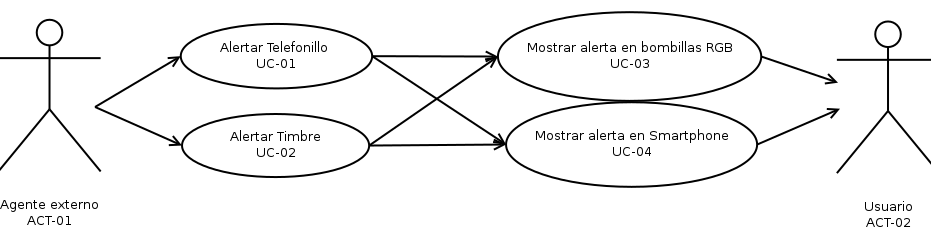
\includegraphics[width=1\textwidth]{casosuso.png}
      \caption{Diagrama de Casos de Uso.}
      \label{casosuso}
    \end{figure}

\clearpage
\section{Definición de actores}

    \begin{table}[!ht]
        \centering
        \resizebox{\textwidth}{!}{%
        \begin{tabular}{|l|p{11cm}|}
            \hline
            \textbf{ACT-01} & Agente externo. \\ \hline
            \textbf{Descripción} & Persona externa al sistema que efectúa la alerta. \\ \hline
        \end{tabular}
        }
        \caption{Actor 01: agente externo.}
        \label{ACT01}
    \end{table}

    \begin{table}[!ht]
        \centering
        \resizebox{\textwidth}{!}{%
        \begin{tabular}{|l|p{11cm}|}
            \hline
            \textbf{ACT-02} & Usuario. \\ \hline
            \textbf{Descripción} & Usuario final del sistema. \\ \hline
        \end{tabular}
        }
        \caption{Actor 02: usuario del sistema.}
        \label{ACT02}
    \end{table}


\section{Requisitos funcionales (Casos de Uso)}

    \begin{table}[!ht]
        \centering
        \resizebox{\textwidth}{!}{%
        \begin{tabular}{|l|p{1cm}|p{9cm}|}
            \hline
            \textbf{UC-01} & \multicolumn{2}{|p{10cm}|}{Alertar telefonillo.} \\ \hline
            \textbf{Objetivos asociados} & \multicolumn{2}{|p{10cm}|}{\vspace{-2mm}\begin{itemize}[noitemsep,nosep]
                                                \item OBJ-02 Alertar a usuario de llamada al telefonillo.
                                            \end{itemize}\vspace{-\baselineskip}\mbox{}} \\ \hline
            \textbf{Requisitos asociados} & \multicolumn{2}{|p{10cm}|}{\vspace{-2mm}\begin{itemize}[noitemsep,nosep]
                                                \item IRQ-01 Información de alertas.
                                            \end{itemize}\vspace{-\baselineskip}\mbox{}} \\ \hline
            \textbf{Descripción} & \multicolumn{2}{|p{10cm}|}{El sistema deberá comportarse tal como se describe en este Caso de Uso cuando un Agente Externo llame al telefonillo.}  \\ \hline
            \textbf{Precondición} & \multicolumn{2}{|p{10cm}|}{Un Agente Externo llama al telefonillo.} \\ \hline
            \textbf{Secuencia normal} & \textbf{Paso} & \textbf{Acción} \\ \cline{2-3} & 1 & Llaman al telefonillo. \\ \cline{2-3} & 2 & Se envía una alerta al sistema. \\ \cline{2-3} & 3 & Se realizan los Casos de Uso UC-03 y UC-04. \\ \hline
            \textbf{Postcondición} & \multicolumn{2}{|p{10cm}|}{Se envía la alerta al sistema.} \\ \hline
            \textbf{Excepciones} & \multicolumn{2}{|p{10cm}|}{Ninguna.} \\ \hline
            \textbf{Rendimiento} & \textbf{Paso} & \textbf{Cota de tiempo} \\ \cline{2-3} & 2 & < 1 segundo. \\ \hline
            \textbf{Comentarios} & \multicolumn{2}{|p{10cm}|}{La frecuencia dependerá de factores externos al sistema que se estudia en el Proyecto.} \\ \hline
        \end{tabular}
        }
        \caption{Caso de Uso 01: Alertar telefonillo.}
        \label{UC01}
    \end{table}

    \begin{table}[!ht]
        \centering
        \resizebox{\textwidth}{!}{%
        \begin{tabular}{|l|p{1cm}|p{9cm}|}
            \hline
            \textbf{UC-02} & \multicolumn{2}{|p{10cm}|}{Alertar timbre.} \\ \hline
            \textbf{Objetivos asociados} & \multicolumn{2}{|p{10cm}|}{\vspace{-2mm}\begin{itemize}[noitemsep,nosep]
                                                \item OBJ-01 Alertar a usuario de llamada al timbre.
                                            \end{itemize}\vspace{-\baselineskip}\mbox{}} \\ \hline
            \textbf{Requisitos asociados} & \multicolumn{2}{|p{10cm}|}{\vspace{-2mm}\begin{itemize}[noitemsep,nosep]
                                                \item IRQ-01 Información de alertas.
                                            \end{itemize}\vspace{-\baselineskip}\mbox{}} \\ \hline
            \textbf{Descripción} & \multicolumn{2}{|p{10cm}|}{El sistema deberá comportarse tal como se describe en este Caso de Uso cuando un Agente Externo llame al timbre de la puerta.}  \\ \hline
            \textbf{Precondición} & \multicolumn{2}{|p{10cm}|}{Un Agente Externo llama al timbre.} \\ \hline
            \textbf{Secuencia normal} & \textbf{Paso} & \textbf{Acción} \\ \cline{2-3} & 1 & Llaman al timbre. \\ \cline{2-3} & 2 & Se envía una alerta al sistema. \\ \cline{2-3} & 3 & Se realizan los Casos de Uso UC-03 y UC-04. \\ \hline
            \textbf{Postcondición} & \multicolumn{2}{|p{10cm}|}{Se envía la alerta al sistema.} \\ \hline
            \textbf{Excepciones} & \multicolumn{2}{|p{10cm}|}{Ninguna.} \\ \hline
            \textbf{Rendimiento} & \textbf{Paso} & \textbf{Cota de tiempo} \\ \cline{2-3} & 2 & < 1 segundo. \\ \hline
            \textbf{Comentarios} & \multicolumn{2}{|p{10cm}|}{La frecuencia dependerá de factores externos al sistema que se estudia en el Proyecto.} \\ \hline
        \end{tabular}
        }
        \caption{Caso de Uso 02: Alertar timbre.}
        \label{UC02}
    \end{table}

    \begin{table}[!ht]
        \centering
        \resizebox{\textwidth}{!}{%
        \begin{tabular}{|l|p{1cm}|p{9cm}|}
            \hline
            \textbf{UC-03} & \multicolumn{2}{|p{10cm}|}{Mostrar alerta en bombilla RGB.} \\ \hline
            \textbf{Objetivos asociados} & \multicolumn{2}{|p{10cm}|}{\vspace{-2mm}\begin{itemize}[noitemsep,nosep]
                                                \item OBJ-01 Alertar a usuario de llamada al timbre.
                                                \item OBJ-02 Alertar a usuario de llamada al telefonillo.
                                            \end{itemize}\vspace{-\baselineskip}\mbox{}} \\ \hline
            \textbf{Requisitos asociados} & \multicolumn{2}{|p{10cm}|}{\vspace{-2mm}\begin{itemize}[noitemsep,nosep]
                                                \item IRQ-01 Información de alertas.
                                            \end{itemize}\vspace{-\baselineskip}\mbox{}} \\ \hline
            \textbf{Descripción} & \multicolumn{2}{|p{10cm}|}{El sistema cambiará el estado de las bombillas RGB de acuerdo a la alerta recibida siempre que estas no ocurran de manera simultánea.}  \\ \hline
            \textbf{Precondición} & \multicolumn{2}{|p{10cm}|}{Se dan uno de los dos Casos de Uso asociados a alertas: UC-01 o UC-02.} \\ \hline
            \textbf{Secuencia normal} & \textbf{Paso} & \textbf{Acción} \\ \cline{2-3} & 1 & Se recibe la alerta en el sistema. \\ \cline{2-3} & 2 & Se almacena el estado de las bombillas RGB. \\ \cline{2-3} & 3 & Se genera alerta luminosa cambiando el estado de las bombillas RGB. \\ \cline{2-3} & 4 & Se regresa al estado previo a la alerta. \\ \hline
            \textbf{Postcondición} & \multicolumn{2}{|p{10cm}|}{El Usuario percibe la alerta.} \\ \hline
            \textbf{Excepciones} & \textbf{Paso} & \textbf{Acción} \\ \cline{2-3} & 1 & Se solapen 2 o más alertas y se omita el aviso. \\ \hline
            \textbf{Rendimiento} & \textbf{Paso} & \textbf{Cota de tiempo} \\ \cline{2-3} & 2 & $\sim$1 segundo. \\ \hline
            \textbf{Comentarios} & \multicolumn{2}{|p{10cm}|}{La frecuencia dependerá de factores externos al sistema que se estudia en el Proyecto.} \\ \hline
        \end{tabular}
        }
        \caption{Caso de Uso 03: Mostrar alerta en bombilla RGB.}
        \label{UC03}
    \end{table}

    \begin{table}[!ht]
        \centering
        \resizebox{\textwidth}{!}{%
        \begin{tabular}{|l|p{1cm}|p{9cm}|}
            \hline
            \textbf{UC-04} & \multicolumn{2}{|p{10cm}|}{Mostrar alerta en smartphone.} \\ \hline
            \textbf{Objetivos asociados} & \multicolumn{2}{|p{10cm}|}{\vspace{-2mm}\begin{itemize}[noitemsep,nosep]
                                                \item OBJ-01 Alertar a usuario de llamada al timbre.
                                                \item OBJ-02 Alertar a usuario de llamada al telefonillo.
                                            \end{itemize}\vspace{-\baselineskip}\mbox{}} \\ \hline
            \textbf{Requisitos asociados} & \multicolumn{2}{|p{10cm}|}{\vspace{-2mm}\begin{itemize}[noitemsep,nosep]
                                                \item IRQ-01 Información de alertas.
                                            \end{itemize}\vspace{-\baselineskip}\mbox{}} \\ \hline
            \textbf{Descripción} & \multicolumn{2}{|p{10cm}|}{El sistema enviará una notificación al smartphone de acuerdo a la alerta recibida siempre que estas no ocurran de manera simultánea.}  \\ \hline
            \textbf{Precondición} & \multicolumn{2}{|p{10cm}|}{Se dan uno de los dos Casos de Uso asociados a alertas: UC-01 o UC-02.} \\ \hline
            \textbf{Secuencia normal} & \textbf{Paso} & \textbf{Acción} \\ \cline{2-3} & 1 & Se recibe la alerta en el sistema. \\ \cline{2-3} & 2 & Se envía la notificación al smartphone. \\ \hline
            \textbf{Postcondición} & \multicolumn{2}{|p{10cm}|}{El Usuario percibe la alerta.} \\ \hline
            \textbf{Excepciones} & \textbf{Paso} & \textbf{Acción} \\ \cline{2-3} & 1 & Se solapen 2 o más alertas y se omita el aviso. \\ \hline
            \textbf{Rendimiento} & \textbf{Paso} & \textbf{Cota de tiempo} \\ \cline{2-3} & 2 & $\sim$1 segundo. \\ \hline
            \textbf{Comentarios} & \multicolumn{2}{|p{10cm}|}{La frecuencia dependerá de factores externos al sistema que se estudia en el Proyecto.} \\ \hline
        \end{tabular}
        }
        \caption{Caso de Uso 04: Mostrar alerta en smartphone.}
        \label{UC04}
    \end{table}

\clearpage
\section{Requisitos no funcionales}

Teniendo en cuenta las restricciones obtenidas a través de las encuestas realizadas, los requisitos no funcionales resultantes son los siguientes:

\begin{description}
    \item[\textbf{NFR–01}:] Se deben utilizar bombillas de luz LED RGB, para generar distintos colores en las alertas.
    \item[\textbf{NFR–02}:] Se debe desarrollar una aplicación para Android en la que se reflejen también las mismas alertas.
\end{description}

Además, según el desarrollo del Proyecto y el estudio de distintas alternativas para la solución final, surgen otros requisitos funcionales:

\begin{description}
    \item[\textbf{NFR–03}:] Las bombillas a utilizar deben ser de rosca E27 (de acuerdo al Informe de diagnóstico del apartado~\ref{sec:informediagnostico}).
    \item[\textbf{NFR-04}:] El nodo central debe ser capaz de manipular peticiones HTTP (de acuerdo a la elección de bombillas en el apartado~\ref{sec:solucionbombillas}).
    \item[\textbf{NFR–05}:] El nodo central debe ser capaz de manipular cadenas JSON (de acuerdo a la elección de bombillas en el apartado~\ref{sec:solucionbombillas}).
\end{description}